\chapter{Introduzione al corso}
%\addcontentsline{toc}{chapter}{Introduzione al corso}

Il primo modulo del corso di Basi di Dati tratterà i seguenti argomenti: algebra relazionale, progettazione di una base di dati, terza forma normale (3NF), organizzazione fisica dei dati e controllo della concorrenza.

\section{Introduzione alle basi di dati}
Un sistema informativo è il componente di un'organizzazione che viene utilizzato per gestire (acquisire, processare, memorizzare, comunicare) le informazioni di interesse. Normalmente opera a supporto delle altre componenti dell'organizzazione ed è indipendente dalla sua computerizzazione.
 
Prima dell'avvento delle basi di dati, ogni applicazione era scritta in un linguaggio orientato alla gestione di file (Cobol,PL/1) e aveva il suo file privato ad organizzazione sequenziale. Ovviamente, un sistema di questo tipo porta con se molti svantaggi tra cui: ridondanza, se due applicazioni usavano gli stessi dati questi venivano replicati; inconsistenza, l'aggiornamento di un dato poteva riguardare una sola copia del dato; dipendenza dei dati, ogni applicazione organizzava i dati tenendo conto dell'uso che doveva farne.

\begin{redbar}
    Una \textbf{Base di Dati} (Database – DB) è un insieme di file mutuamente connessi. Questi insiemi sono organizzati in diverse strutture dati che ne facilitano la creazione, l'accesso e l'aggiornamento ed ottimizzano la gestione delle risorse fisiche. Quindi l'obiettivo di una base di dati è facilitare l'elaborazione dei dati sulla base delle loro relazioni.
\end{redbar}

\begin{redbar}
    I \textbf{Sistemi di Gestione di Basi di Dati} (Database Management System – DBMS) sono strumenti software per la gestione di grandi masse (strutturate, processabili, condivise) di dati residenti su memoria secondaria.
\end{redbar}

Quando si registrano dei dati in formato elettronico si possono avere dei dati strutturati oppure dei dati non strutturati. I \textit{dati strutturati} possono essere rappresentati dalle strutture dati gestite da un programma (stringhe, numeri...), mentre quelli \textit{non strutturati} sono quei testi scritti in un linguaggio naturale. L'utilità nell'utilizzo dei dati strutturati proviene dal fatto che si può accedere singolarmente agli elementi della struttura tramite "interrogazioni" per recuperare le informazioni necessarie, oppure si possono effettuare dei calcoli sui dati stessi.

Una base di dati è una risorsa integrata condivisa da diverse componenti e, l'integrazione e la condivisione, permettono di ridurre le ridondanze e le inconsistenze dei dati. Da notare che la condivisione dei dati non è mai completa (controllo della privacy e regolamentazione degli accessi) e comporta la necessità di gestire accessi contemporanei agli stessi dati (controllo della concorrenza).

Nelle basi di dati possiamo distinguere i modelli logici da quelli concettuali. I \textit{modelli logici} ci permettono di astrarre dall'organizzazione fisica, in fase di progettazione, invece, occorre avere dei \textit{modelli concettuali} che ci permettono di rappresentare le entità del mondo reale e le loro relazioni.

Ogni database contiene tre livelli di astrazione (vedi Figura \ref{fig:db-astrazione}): uno \textit{schema interno}, ovvero il modo in cui vengono memorizzate le tabelle e gli indici nei file, è chiamato anche schema fisico che rappresenta la distribuzione dei dati su disco; lo \textit{schema logico} è la descrizione dell'intera base di dati nel modello principale del DBMS; gli \textit{schemi esterni} sono la descrizione di una porzione della base di dati attraverso viste parziali che riflettono esigenze e privilegi di accesso di particolari tipologie di utenti. Gli accessi alla base di dati avvengono solamente attraverso lo schema esterno.

\begin{figure}
    \centering
    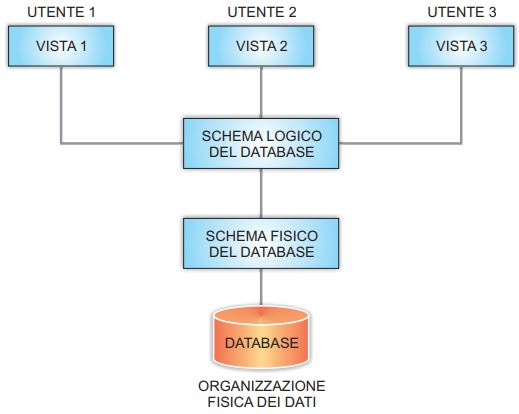
\includegraphics[width=0.5\linewidth]{images/db-astrazione.JPG}
    \caption{Livelli di astrazione dei sistemi per database}
    \label{fig:db-astrazione}
\end{figure}

Per le basi di dati esistono un \textit{data definition language} (DDL), un linguaggio per la definizione di schemi (logici, esterni, fisici) e altre operazioni generali, e un \textit{data manipulation language} (DML), un linguaggio per l'interrogazione e l'aggiornamento di istanze di basi di dati. L'SQL (Structured Query Language) è un linguaggio standardizzato per database basati sul modello relazionale (RDBMS). In SQL i due tipi di funzionalità sono integrate in un unico linguaggio di comandi.

\section{Storia delle basi di dati}
I primi database gerarchici, progettati dalla IBM, furono usati nel progetto Apollo del 1964, mentre il primo database in commercio, DL/1, arriva qualche anno più tardi. Vengono chiamati database gerarchici perché prevedono delle gerarchie tra i dati con dei puntamenti tramite indirizzi fisici, la struttura di un database gerarchico è quella di un albero dove ogni nodo ha solo un genitore. Con l'avvento dei database a rete è possibile rappresentare un maggior numero di relazioni, con la rappresentazione dei dati tramite una collezione di record di tipo omogeneo, e con l'implementazione dei puntatori come relazioni binarie. Il modello di un database reticolare è rappresentato da una struttura a grafo dove i nodi sono i record e gli archi sono le relazioni. Nel 1970, con il modello di Codd, si introduce il modello relazionale dove i dati e le relazioni sono rappresentati come valori univoci di un record.
Verso la metà dei anni '80 arrivarono i primi database orientati agli oggetti.

